
\section{Independent Component Analysis} \label{sec:ICA}
Independent component analysis has proven to be a very useful tool in separating noise from wanted signal in many applications. The following section will seek to elucidate the general basic theoretical background behind the blind source separation analysis.  

The basic idea about Independent Component Analysis (ICA) is to recover $m$ signal sources, which are mixed in $n$ observed signals. The observed signal is given by \cite{Hyvarinen2001}:
\begin{equation}
\mathbf{x} = \mathbf{A}\mathbf{s}
\end{equation}
where \textbf{x} is a observed signal vector containing the mixed signal elements $x_1, x_2, ..., x_n$, \textbf{s} is the source signal vector with the elements $s_1, s_2, ..., s_m$ and $\mathbf{A}$ is a mixing matrix with the dimension $n \times m$. Note that the dimensions of the mixing matrix can be equal to each other, meaning that it is required to have at least the number of observed signals as the source signals. The observed signal is assumed to be a linear mix of independent source signals. When performing ICA the goal is to find an inverted mixing matrix \textbf{$A^{-1}$} that recovers the source signal \cite{Hyvarinen2001}:
\begin{equation}
\mathbf{s} = \mathbf{A^{-1}}\mathbf{x}
\end{equation}
This can easily be achieved if the mixing matrix is known. However, this is rarely the case, as both the mixing matrix and source signals are unknown. There is no reliable way, to fully determine \textbf{s}, thus a set of assumptions are required, which the ICA method is based on \cite{Hyvarinen2001}:
\begin{itemize}
	\item The independent components (IC)’s are assumed to be statistically independent.
	\item The IC’s must be non-Gaussian distributions.
\end{itemize}
Regarding the assumption of independence, a set of variables $y_1, y_2, ..., y_n$ is not allowed to share mutual information so that $i \neq j$. This can be expressed as the joint probability of the variables is equal the product of each marginal probability of the variables \cite{Hyvarinen2001}:
\begin{equation}
p(y_1, y_2, …, y_n) = p(y_1) \cdot p(y_2) \cdot ... \cdot p(y_n) 
\end{equation} \label{eq:independence}
Satisfying this condition assures independency of the variables. A graphical example of independence in two dimensions is shown in \figref{fig:back:independence} \cite{Hyvarinen2001, Hyvarinen2000}. 

\begin{figure}[H]                 
	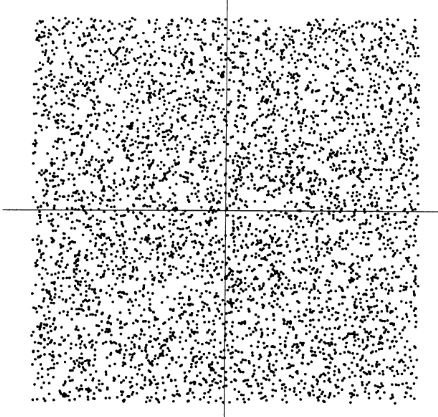
\includegraphics[width=.35\textwidth]{figures/aBackground/independence}  
	\caption{Figure illustrating the joint distribution of two independent components having uniform distribution. \cite{Hyvarinen2000}.}
	\label{fig:back:independence} 
\end{figure}

It is clear to see that information about a variable on the horizontal axis does not give any information about variables at vertical axis and vice versa.  Note that uncorrelatedness does not equal independency. However, whitening of the observed signals and thus ensuring uncorrelatedness is very helpful in solving the ICA problem. Whitening of the data is archived by performing a linear transformation that transforms the components so that the covariance matrix equals the identity matrix, thus having unit-variance. 
This can be expressed through performing a linear transformation of \textbf{x} into a random vector \textbf{z}:

\begin{equation}
\mathbf{z} = \mathbf{V}\mathbf{x} = \mathbf{V}\mathbf{A}\mathbf{s} 
\end{equation}
A graphical example of whitened data in two dimensions is shown in \figref{fig:back:whitening}  \cite{Hyvarinen2001,Hyvarinen2000}.

\begin{figure}[H]                 
	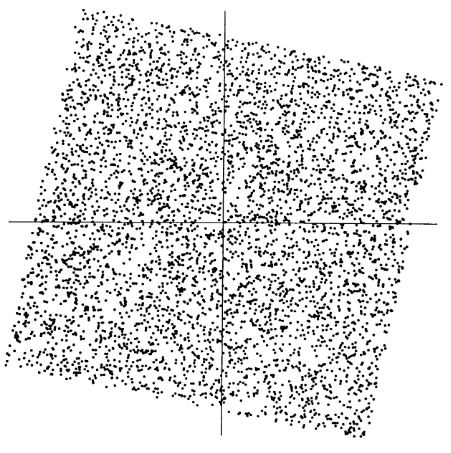
\includegraphics[width=.35\textwidth]{figures/aBackground/whitening}  
	\caption{Figure illustrating the impact of whitening on the joint distribution of two components \cite{Hyvarinen2000}.}
	\label{fig:back:whitening} 
\end{figure}

The squared distribution is clearly a rotated form of the independent data. What is left to ensure independence and solving the ICA problem is to estimate an angle that gives the correct rotation.
Concerning the second assumption on non-Gaussianity, the joint distribution of uncorrelated Gaussian distributions are not necessarily independent, and the distribution will be symmetrical and no information on the direction of the distribution can be derived. Thus, no transformation that allows independency can be performed, and the mixing matrix \textbf{A} can not be estimated from the mixtures. This can be shown in a two dimensional example with two sources $s_1$ and $s_2$ and the mixing matrix \textbf{A}, the joint probability density function (pdf) of Gaussian distributions is calculated as \cite{Hyvarinen2001}:
\begin{equation} \label{using this?}
\begin{split}
p(s_1,s_2) & = \frac{1}{2\pi}exp(-\frac{s^{2}_{1}+s^{2}_{2}}{2}) \\
& = \frac{1}{2\pi}exp(-\frac{\parallel \mathbf{s} \parallel ^2}{2}) 
\end{split}
\end{equation}
%\begin{equation}
%p(s_1,s_2) = \frac{1}{2\pi}exp(-\frac{s^{2}_{1}+s^{2}_{2}}{2}) 
%\end{equation}
%\begin{equation}
%= \frac{1}{2\pi}exp(-\frac{\parallel \mathbf{s} \parallel ^2}{2}) 
%\end{equation}
For an orthogonal mixing matrix \textbf{A} the inverse can be written as $\mathbf{A^{-1}} = \mathbf{{A^T}}$, and then $\mathbf{{s} = \mathbf{A^T} \mathbf{x}}$. The joint pdf can then be rewritten as:
\begin{equation}
p(x_1,x_2) = \frac{1}{2\pi}exp(-\frac{\parallel \mathbf{A^T} \mathbf{x} \parallel ^2}{2}) \mid Det (\mathbf{A^T}) \mid
\end{equation}
Because ${\parallel \mathbf{A^T} \mathbf{x} \parallel ^2} = \parallel \mathbf{x} \parallel ^2$ and $\mid Det ( \mathbf{A^T} ) \mid = 1$, hence the orthogonality of \textbf{A}, the joint pdf is:
\begin{equation}
p(x_1,x_2) = \frac{1}{2\pi}exp(-\frac{\parallel \mathbf{s} \parallel ^2}{2}) 
\end{equation}
The joint pdf is not changed when choosing an orthogonal mixing matrix as well as the property of independence. No further information about the mixing matrix can thus be revealed when the source signals are from a Gaussian distribution. \cite{Hyvarinen2001}

\subsection{ICA approaches}
As the mixing matrix and source signal most often are unknown, the IC’s must be approximated in an iterative process. There are two main ICA iteration approaches: minimizing mutual information and maximizing non-Gaussianity. The former approach seeks to minimize mutual information by maximizing independence between components. In practice this is done by minimizing the difference between the joint density distribution and the product of the marginal density functions, the left-hand side and right-hand side of \eqref{eq:independence}. This can for instance be done through a Kullback-Leibler divergence between the $p(y_1,y_2)$ and $p(y_1)*p(y_2)$ in a two dimensional case.
The second approach seeks to maximize non-Gaussianity of the components. The central limit theorem states that if sources are mixed, the mix tend to get more Gaussian than the individual sources. The strategy here is to find the directions in the data that is as far away from Gaussian as possible through a linear transformation. That direction will most likely be independent components. To find these directions different ICA approaches use fourth order moments and negentropy of the data. \cite{Hyvarinen2001} 
